
%% $Id$

\chapter{Presenting theories}

Isabelle provides several ways to present the outcome of formal developments,
including WWW-based browsable libraries or actual printable documents.
Presentation is centered around the concept of \emph{logic sessions}.  The
structure of sessions is that of a tree, with Isabelle \texttt{Pure} at its
root, further derived object-logics (e.g.\ \texttt{HOLCF} from \texttt{HOL},
and \texttt{HOL} from \texttt{Pure}), and application sessions at its leaves.
The latter usually do not have a separate {\ML} image.

The \texttt{usedir} utility (see \S\ref{sec:tool-usedir}) provides the prime
means for managing Isabelle sessions, including proper setup for presentation.


\section{Generating theory browsing information} \label{sec:info}
\index{theory browsing information|bold}

As a side-effect of running a logic sessions, Isabelle is able to generate
theory browsing information, including HTML documents that show a theory's
definition, the theorems proved in its ML file and the relationship with its
ancestors and descendants.  Besides the HTML file that is generated for every
theory, Isabelle stores links to all theories in an index file. These indexes
are linked with other indexes to represent the tree structure of Isabelle's
logics.

Isabelle also generates graph files that represent the theory hierarchy of a
logic.  There is a graph browser Java applet embedded in the generated HTML
pages, and also a stand-alone application that allows browsing theory graphs
without having to start a WWW browser first.  The latter version also includes
features such as generating {\sc PostScript} files, which are not available in
the applet version.  See \S\ref{sec:browse} for further information.

\medskip

In order to let Isabelle generate theory browsing information for logics that
are part of the Isabelle distribution, simply append ``\texttt{-i true}'' to
the \settdx{ISABELLE_USEDIR_OPTIONS} setting before making a logic.  For
example, in order to do this for {\FOL}, add something like this to your
Isabelle settings file
\begin{ttbox}
ISABELLE_USEDIR_OPTIONS="-i true"
\end{ttbox}
and then change into the \texttt{src/FOL} directory of the Isabelle
distribution and run \texttt{isatool make}, or even \texttt{isatool make all}.

Some sessions (such as \texttt{HOL/Isar_examples}) even provide actual
printable documents.  These are prepared automatically as well if enabled by
giving an appropriate \texttt{-d} option, e.g.\
\begin{ttbox}
ISABELLE_USEDIR_OPTIONS="-i true -d dvi"
\end{ttbox}
See \S\ref{sec:tool-document} for further information on Isabelle document
preparation.

\bigskip The theory browsing information is stored within the directory
determined by the \settdx{ISABELLE_BROWSER_INFO} setting.  The
\texttt{index.html} file located there provides an entry point to all standard
Isabelle logics.  A complete HTML version of all object-logics and examples of
the Isabelle distribution is available at
\begin{center}\small
  \begin{tabular}{l}
    \url{http://www.cl.cam.ac.uk/Research/HVG/Isabelle/library/} \\
    \url{http://isabelle.in.tum.de/library/} \\
  \end{tabular}
\end{center}

\medskip

The generated HTML document of any theory includes all theorems proved in the
corresponding {\ML} file, provided these have been stored properly via
\ttindex{qed}, \ttindex{qed_goal}, \ttindex{qed_goalw}, \ttindex{bind_thm},
\ttindex{bind_thms} or \ttindex{store_thm}.  Section headings may be included
in the presentation via the {\ML} function
\begin{ttbox}\index{*section}
section: string -> unit
\end{ttbox}

\medskip

In order to present your own theories on the web, simply copy the whole
\texttt{ISABELLE_BROWSER_INFO} directory to your WWW server, after generating
browser info like this:
\begin{ttbox}
isatool usedir -i true HOL Foo
\end{ttbox}
This assumes that directory \texttt{Foo} contains some \texttt{ROOT.ML} file
to load all your theories, and {\HOL} is your parent logic image.  Ideally,
theory browser information would have been generated for {\HOL} already.

Alternatively, one may specify an external link to an existing body of HTML
data by giving \texttt{usedir} a \texttt{-P} option like this:
\begin{ttbox}
isatool usedir -i true -P http://isabelle.in.tum.de/library/ HOL Foo
\end{ttbox}



\section{Browsing theory graphs} \label{sec:browse}
\index{theory graph browser|bold} 

The graph browser is a tool for visualizing dependency graphs of
Isabelle theories. Certain nodes of the graph (i.e.~theories) can be
grouped together in ``directories'', whose contents may be hidden,
thus enabling the user to filter out irrelevant information.  The
browser is written in Java, it can be used both as a stand-alone
application and as an applet.


\subsection{Invoking the graph browser}

The stand-alone version of the graph browser is wrapped up as an
Isabelle tool called \tooldx{browser}:
\begin{ttbox}
Usage: browser [GRAPHFILE]
\end{ttbox}
When no filename is specified, the browser automatically changes to
the directory \texttt{ISABELLE_BROWSER_INFO/graph/data}.

\medskip The applet version of the browser can be invoked by opening the {\tt
  index.html} file in the directory \texttt{ISABELLE_BROWSER_INFO} from your
Web browser and selecting ``version for Java capable browsers''.  There is
also a link to the corresponding theory graph in every logic's {\tt
  index.html} file.


\subsection{Using the graph browser}

The browser's main window, which is shown in figure
\ref{browserwindow}, consists of two sub-windows: In the left
sub-window, the directory tree is displayed. The graph itself is
displayed in the right sub-window.
\begin{figure}[ht]
  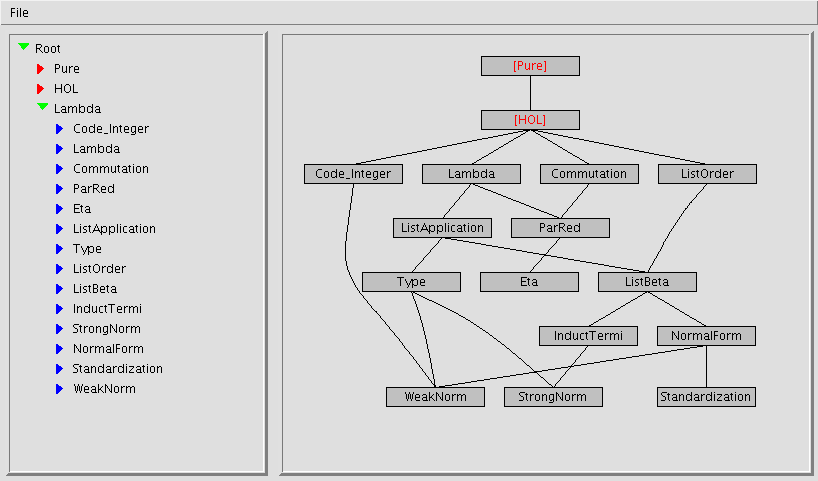
\includegraphics[width=\textwidth]{browser_screenshot}
  \caption{\label{browserwindow} Browser main window}
\end{figure}


\subsubsection*{The directory tree window}

This section describes the usage of the directory browser and the
meaning of the different items in the browser window.
\begin{itemize}
  
\item A red arrow before a directory name indicates that the directory
  is currently ``folded'', i.e.~the nodes in this directory are
  collapsed to one single node. In the right sub-window, the names of
  nodes corresponding to folded directories are enclosed in square
  brackets and displayed in red color.
  
\item A green downward arrow before a directory name indicates that
  the directory is currently ``unfolded''. It can be folded by
  clicking on the directory name.  Clicking on the name for a second
  time unfolds the directory again.  Alternatively, a directory can
  also be unfolded by clicking on the corresponding node in the right
  sub-window.
  
\item Blue arrows stand before ordinary node (i.e.~theory) names. When
  clicking on such a name, the graph display window focuses to the
  corresponding node. Double clicking invokes a text viewer window in
  which the contents of the theory file are displayed.

\end{itemize}


\subsubsection*{The graph display window}

When pointing on an ordinary node, an upward and a downward arrow is
shown.  Initially, both of these arrows are green. Clicking on the
upward or downward arrow collapses all predecessor or successor nodes,
respectively. The arrow's color then changes to red, indicating that
the predecessor or successor nodes are currently collapsed. The node
corresponding to the collapsed nodes has the name ``{\tt [....]}''. To
uncollapse the nodes again, simply click on the red arrow or on the
node with the name ``{\tt [....]}''. Similar to the directory browser,
the contents of theory files can be displayed by double clicking on
the corresponding node.


\subsubsection*{The ``File'' menu}

Please note that due to Java security restrictions this menu is not
available in the applet version. The meaning of the menu items is as
follows:
\begin{description}
  
\item[Open$\ldots$] Open a new graph file.
  
\item[Export to PostScript] Outputs the current graph in {\sc
    PostScript} format, appropriately scaled to fit on one single
  sheet of paper.  The resulting file can printed directly.
  
\item[Export to EPS] Outputs the current graph in Encapsulated {\sc
    PostScript} format. The resulting file can be included in other
  documents.

\item[Quit] Quit the graph browser.

\end{description}


\subsection*{*Syntax of graph definition files}

A graph definition file has the following syntax:
\begin{eqnarray*}
  \mbox{\it graph} & = & \{ \: \mbox{\it vertex \tt ;} \: \} ^ + \\
  vertex & = & \mbox{\it vertexname} \: \mbox{\it vertexID} \: \mbox{\it dirname} \: [ \mbox{\tt +} ]
  \: \mbox{\it path} \: [ \mbox{\tt <} | \mbox{\tt >} ] \: \{ \: \mbox{\it vertexID} \: \} ^ *
\end{eqnarray*}

The meaning of the items in a vertex description is as follows:
\begin{description}
  
\item[vertexname] The name of the vertex.
  
\item[vertexID] The vertex identifier. Note that there may be two
  vertices with equal names, whereas identifiers must be unique.
  
\item[dirname] The name of the ``directory'' the vertex should be
  placed in.  A ``{\tt +}'' sign after {\it dirname} indicates that
  the nodes in the directory are initially visible. Directories are
  initially invisible by default.
  
\item[path] The path of the corresponding theory file. This is
  specified relatively to the path of the graph definition file.
  
\item[List of successor/predecessor nodes] A ``{\tt <}'' sign before
  the list means that successor nodes are listed, a ``{\tt >}'' sign
  means that predecessor nodes are listed. If neither ``{\tt <}'' nor
  ``{\tt >}'' is found, the browser assumes that successor nodes are
  listed.

\end{description}


\section{Preparing Isabelle session documents --- \texttt{isatool document}}
\label{sec:tool-document}

The \tooldx{document} utility prepares logic session documents, processing the
sources both provided by the user and generated by Isabelle.  Its usage is:
\begin{ttbox}
Usage: document [OPTIONS] [DIR]

  Options are:
    -o FORMAT    specify output format: dvi (default), dvi.gz, ps,
                 ps.gz, pdf

  Prepare the theory session document in DIR (default '.')
  producing the specified output format.
\end{ttbox}
This tool is usually run automatically as part of the corresponding session,
provided document preparation is enabled (cf.\ the \texttt{-d} option of the
\texttt{usedir} utility, \S\ref{sec:tool-usedir}).  It may be manually invoked
on the generated browser information document output as well.

\medskip Document preparation requires a properly setup ``\texttt{document}''
directory within the logic session sources.  This directory is supposed to
contain all the files needed to produce the actual document, apart from the
actual theories as generated by Isabelle.

\medskip For simple documents, the \texttt{document} tool is smart enough to
create any of the output formats, taking \texttt{root.tex} supplied by the
user as a starting point.  This even includes multiple runs of {\LaTeX} to
accommodate references and bibliographies (the latter assumes
\texttt{root.bib} within the same directory).

For complex documents, a separate \texttt{IsaMakefile} may be given instead.
It should provide targets for any admissible document format; these have to
produce corresponding output files named after \texttt{root} as well, e.g.\ 
\texttt{root.dvi} for target format \texttt{dvi}.

\medskip When running the session, Isabelle copies the original
\texttt{document} directory into its proper place within
\texttt{ISABELLE_BROWSER_INFO} according to the session path.  Then, for any
processed theory $A$ some {\LaTeX} source is generated and put there as
$A$\texttt{.tex}.  Furthermore, a list of all generated theory files is put
into \texttt{session.tex}.  Typically, the root {\LaTeX} file provided by the
user would include \texttt{session.tex} to get a document containing all the
theories.

The {\LaTeX} versions of the theories require some macros defined in
\texttt{isabelle.sty} as distributed with Isabelle.  Doing
\verb,\usepackage{isabelle}, somewhere in \texttt{root.tex} should work fine;
the underlying Isabelle \texttt{latex} utility already includes an appropriate
{\TeX} inputs path.  For proper setup of hyperlinks and bookmarks in PDF
documents we recommend to include \verb,pdfsetup.sty, as well.\footnote{It is
  safe to do so even without using PDF~\LaTeX.}

\medskip As a final step, \texttt{isatool document} is run on the resulting
\texttt{document} directory.  Thus the actual output document is built and
installed in its proper place (as linked by the session's
\texttt{index.html}).  Note that the generated sources are left as is.  While
they may be safely deleted afterwards, this is \emph{not} done automatically.


\section{Running {\LaTeX} within the Isabelle environment --- \texttt{isatool latex}}
\label{sec:tool-latex}

The \tooldx{latex} utility provides the basic interface for Isabelle document
preparation.  Its usage is:
\begin{ttbox}
Usage: latex [OPTIONS] [FILE]

  Options are:
    -o FORMAT    specify output format: dvi (default), dvi.gz, ps,
                 ps.gz, pdf, or bbl

  Run LaTeX (and related tools) on FILE (default root.tex),
  producing the specified output format.
\end{ttbox}
Appropriate {\LaTeX}-related programs are run on the input file, according to
the given output format: \texttt{latex}, \texttt{pdflatex}, \texttt{bibtex},
\texttt{dvips}.  The actual commands are determined from the settings
environment (see \texttt{ISABELLE_LATEX} etc.).

It is important to note that the {\LaTeX} inputs file space has to be properly
setup to include the Isabelle styles.  Usually, this may be done by modifying
the \settdx{TEXINPUTS} variable in settings like this:
\begin{ttbox}
TEXINPUTS="$ISABELLE_HOME/lib/texinputs:$TEXINPUTS"
\end{ttbox}
This is known to work with recent versions of the \textsl{teTeX} distribution.



\section{Managing logic sessions --- \texttt{isatool usedir}} \label{sec:tool-usedir}

The \tooldx{usedir} utility builds object-logic images, or runs example
sessions based on existing logics. Its usage is:
\begin{ttbox}
Usage: usedir LOGIC NAME

  Options are:
    -B           build mode with THIS_IS_ISABELLE_BUILD indication
    -P PATH      set path for remote theory browsing information
    -b           build mode (output heap image, using current dir)
    -d FORMAT    build document as FORMAT (default false)
    -i BOOL      generate theory browsing information,
                 i.e. HTML / graph data (default false)
    -r           reset session path
    -s NAME      override session NAME

  Build object-logic or run examples. Also creates browsing
  information (HTML etc.) according to settings.

  ISABELLE_USEDIR_OPTIONS=
\end{ttbox}

Note that the value of the \settdx{ISABELLE_USEDIR_OPTIONS} setting is
implicitly prefixed to \emph{any} \texttt{usedir} call. Since the
\ttindex{IsaMakefile}s of all object-logics distributed with Isabelle just
invoke \texttt{usedir} for the real work, one may control compilation options
globally via above variable. In particular, generation of \rmindex{HTML}
browsing information and document preparation is controlled this way.


\subsection*{Options}

Basically, there are two different modes of operation: \emph{build
  mode} (enabled through the \texttt{-b} option) and \emph{example
  mode} (default).

Calling \texttt{usedir} with \texttt{-b} runs \texttt{isabelle} with input
image \texttt{LOGIC} and output to \texttt{NAME}, as provided on the command
line. This will be a batch session, running \texttt{ROOT.ML} from the current
directory and then quitting.  It is assumed that \texttt{ROOT.ML} contains all
{\ML} commands required to build the logic.  The \texttt{-B} option is like
\texttt{-b}, but also indicates \texttt{THIS_IS_ISABELLE_BUILD=true} via the
process environment.  This usually causes the \texttt{ISABELLE\_OUTPUT} and
\texttt{ISABELLE_BROWSER_INFO} settings to refer to some location within the
Isabelle distribution directory, rather than the user's home directory.

In example mode, \texttt{usedir} runs a read-only session of \texttt{LOGIC}
(typically just built before) and automatically runs \texttt{ROOT.ML} from
within directory \texttt{NAME}.  It assumes that file \texttt{ROOT.ML} in
directory \texttt{NAME} contains appropriate {\ML} commands to run the desired
examples.

\medskip The \texttt{-i} option controls theory browsing data generation. It
may be explicitly turned on or off --- the last occurrence of \texttt{-i} on
the command line wins.  The \texttt{-P} option specifies a path (or actual
URL) to be prefixed to any \emph{non-local} reference of existing theories.
Thus user sessions may easily link to existing Isabelle libraries already
present on the WWW.

\medskip The \texttt{-d} option controls document preparation.  Valid
arguments are \texttt{false} (do not prepare document; this is default), or
any of \texttt{dvi}, \texttt{dvi.gz}, \texttt{ps}, \texttt{ps.gz},
\texttt{pdf}.  The logic session has to provide a properly setup
\texttt{document} directory.  See \S\ref{sec:tool-document} and
\S\ref{sec:tool-latex} for more details.

\medskip Any \texttt{usedir} session is named by some \emph{session
  identifier}. These accumulate, documenting the way sessions depend
on others. For example, consider \texttt{Pure/FOL/ex}, which refers to
the examples of {\FOL} which is built upon {\Pure}.

The current session's identifier is by default just the base name of
the \texttt{LOGIC} argument (in build mode), or of the \texttt{NAME}
argument (in example mode). This may be overridden explicitely via the
\texttt{-s} option.


\subsection*{Examples}

Refer to the \texttt{IsaMakefile}s of the Isabelle distribution's
object-logics as a model for your own developments.  For example, see
\texttt{src/FOL/IsaMakefile}.


%%% Local Variables: 
%%% mode: latex
%%% TeX-master: "system"
%%% End: 
